\section{Studies with simulated data}

\subsection{Single Pulse Simulations}

The studies with the network were first conducted on simulated data to fine-tune the network before studying the impact on real data.
Pulses were generated using a Landau function on top of a flat background. 
\begin{equation}
L(x)=e^{-\frac{1}{2}(\frac{x-x_0}{\sigma} + e^{\frac{x-x_0}{\sigma}}) }
%(\frac{x-x_0}{$sigma} + e^{\frac{x-x_0}{$sigma}}})
\end{equation}

For each sample the position of the peak ($x_0$) was generated using a pseudo-random generator and the sigma value of 0.015 was used (which is similar to the pulses we see from the detectors).
A large training sample was used to train the autoencoder and a validation sample (also randomly generated) was used to compare the output from the network to the original pulse shape. For our initial studies, the network architecture [48,24,12,24,48] was used with {\bf ReLU} activation functions for hidden layers and {\bf Linear} activation function for the output layer.
The results are shown in Figure~\ref{fig:results_sp_48}. 

\begin{figure}[h!]
\centering
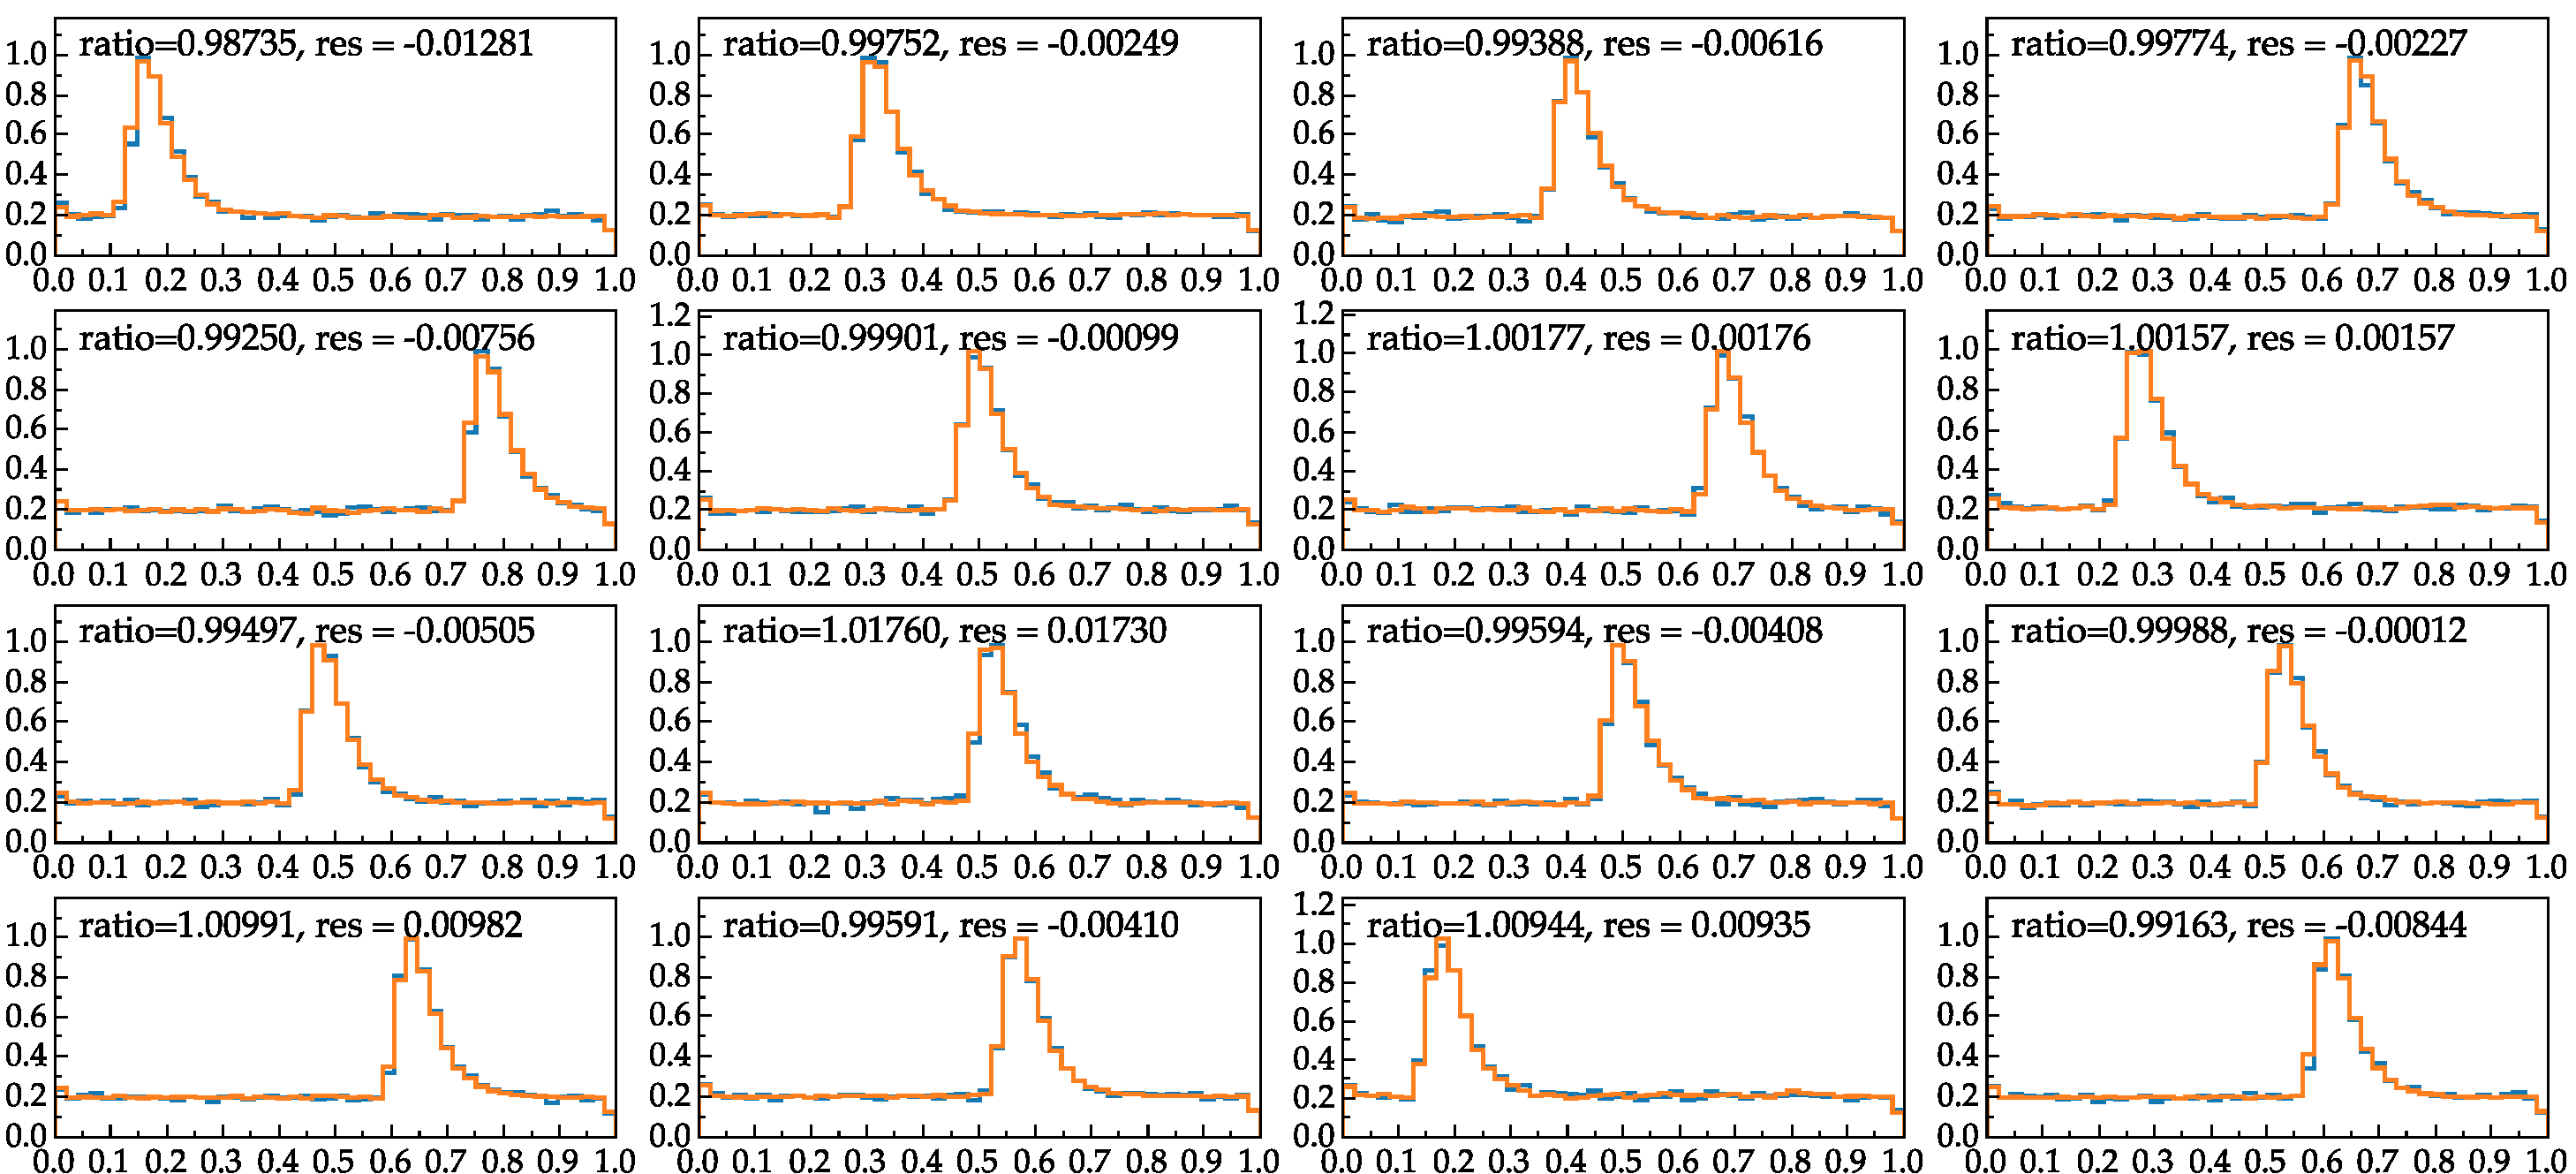
\includegraphics[width=0.9\columnwidth]{results_sp_48.pdf}
\caption{Original pulses plotted with reconstructed pulses overlayed. The data is produced by simulating a single pulse in the 48-bin region.} 
\label{fig:results_sp_48}
\end{figure}

It can be seen from the figure that the decoder reconstructs the pulses from encoded data with great accuracy, and the stored data is 4 times smaller (vector of the length 12 for the middle layer).
In Figure~\ref{fig:results_sp_48_res} (left) the distribution of the normalized difference of the pulse integral is plotted for the validation sample. As can be seen from the figure the reconstructed from the encoding pulse integral is on average in agreement with the input pulse with a resolution of about $0.7\%$. In Figure~\ref{fig:results_sp_48_res} (right) the time difference is calculated for the original pulse and the decompressed pulse. The time is calculated assuming that the 48 bins in the pulse represent a timing window of $48~ns$, the resulting difference is multiplied by $1000$ and the difference is given in pico-seconds.

\begin{figure}[h!]
\centering
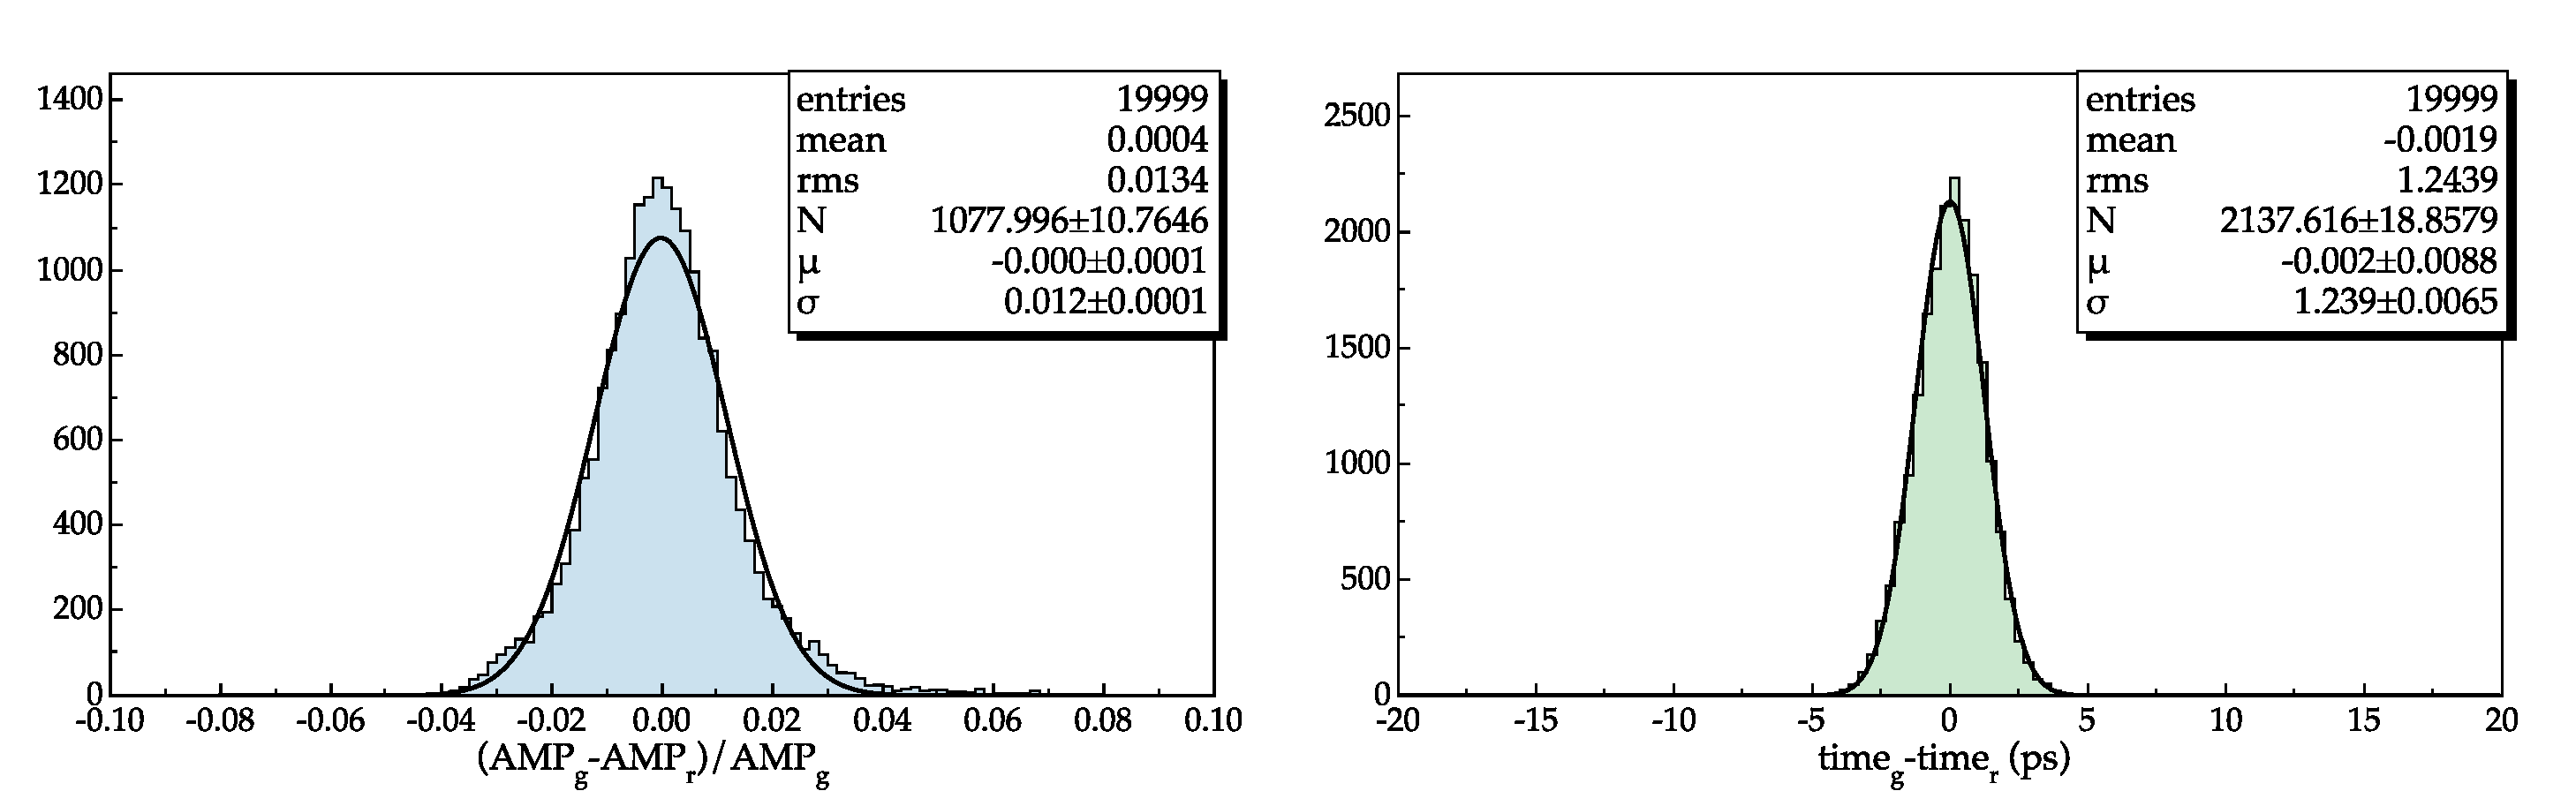
\includegraphics[width=0.9\columnwidth]{out_evaluate_csv_single_24.pdf}
\caption{The resolution of the pulse integrals. The integral of the pulse is compared to the integral calculated from decompressed pulses (on the right), and time calculated from the original pulse is compared to the time calculated from the decompressed pulse.} 
\label{fig:results_sp_48_res}
\end{figure}

In real experimental conditions, it is not uncommon to have two pulses in a given time window when the electronics are being read. Our next study is to use the same network architecture for training a network for compressing two pulse inputs.

\subsection{Double Pulse Simulations}

To study the compression of double pulse data we generated a new sample consisting of two pulses with random mean positions and random height ratios, the width of the pulse was kept the same (with $\sigma=0.015$). The results of compression and decompression for two pulse data are shown in Figure~\ref{fig:results_dp_48}. It can be seen from the figure that the network is able to accurately reconstruct the peak positions but in some cases, the heights and the widths of the peaks do not match the input peak, which leads to degraded accuracy for peak integral calculations. 

\begin{figure}[h!]
\centering
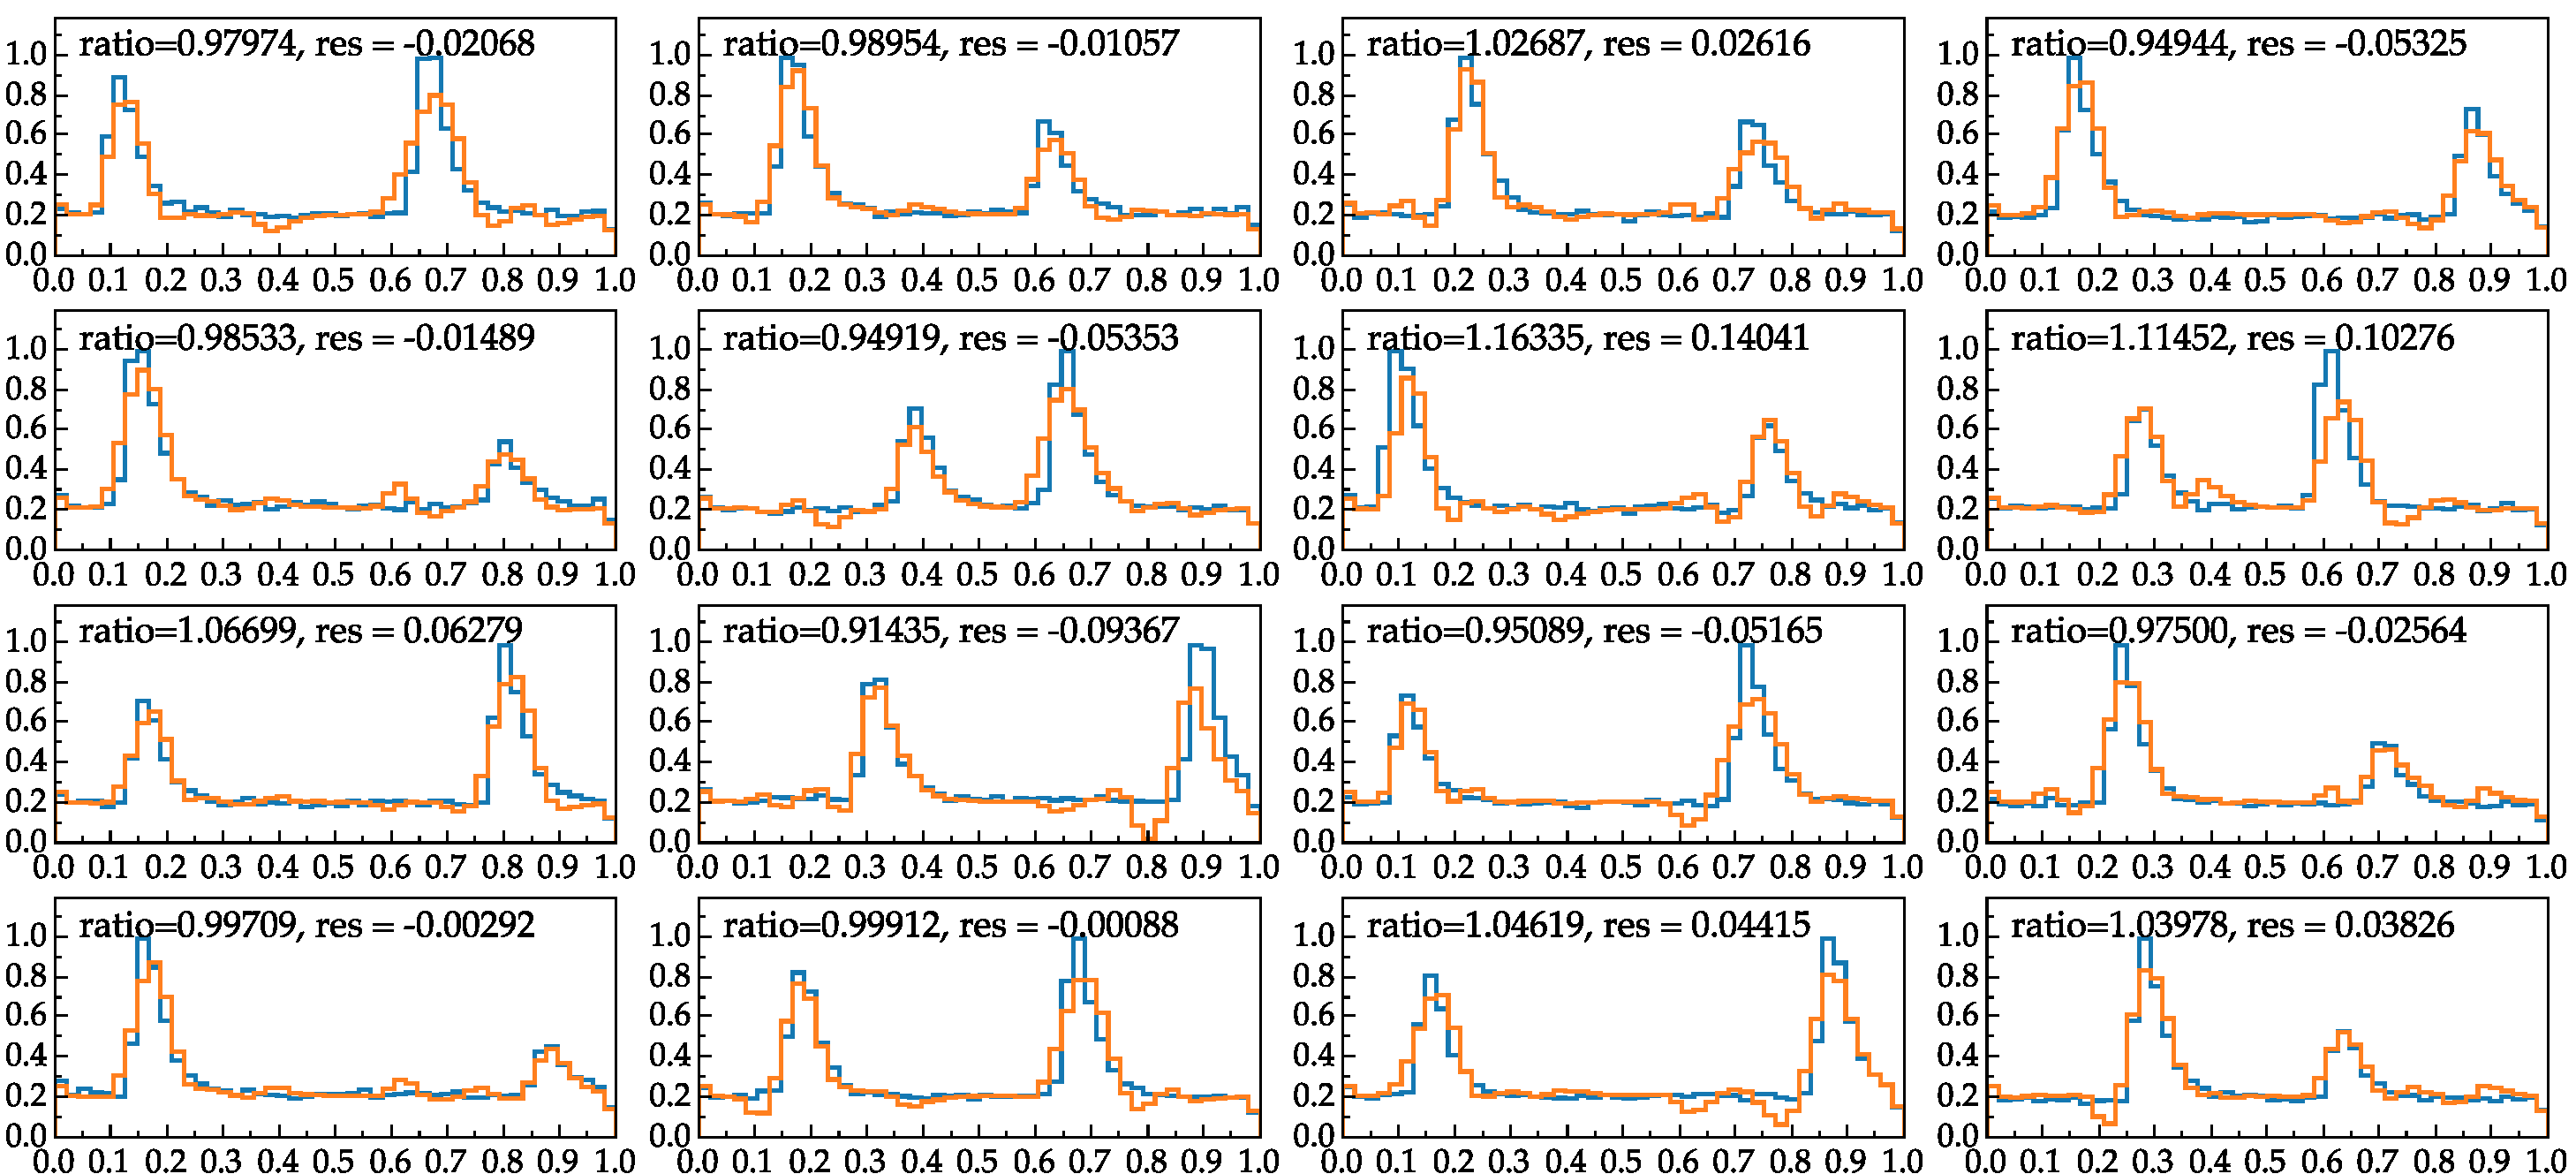
\includegraphics[width=0.9\columnwidth]{results_dp_48.pdf}
\caption{Generated double pulses plotted with the decompressed pulses overlayed. The compression is done with the original auto-encoder [48,24,24,12,24,24,48] architecture. The data is produced by simulating a single pulse in the 48-bin region.} 
\label{fig:results_dp_48}
\end{figure}

The average resolution for the peak integral reconstruction is shown in Figure~\ref{fig:results_dp_48_res}, and is about $4\%$. It's worth mentioning that the heights of the peaks being reconstructed with degraded accuracy can lead to inaccurate pulse timing calculations.

\begin{figure}[h!]
\centering
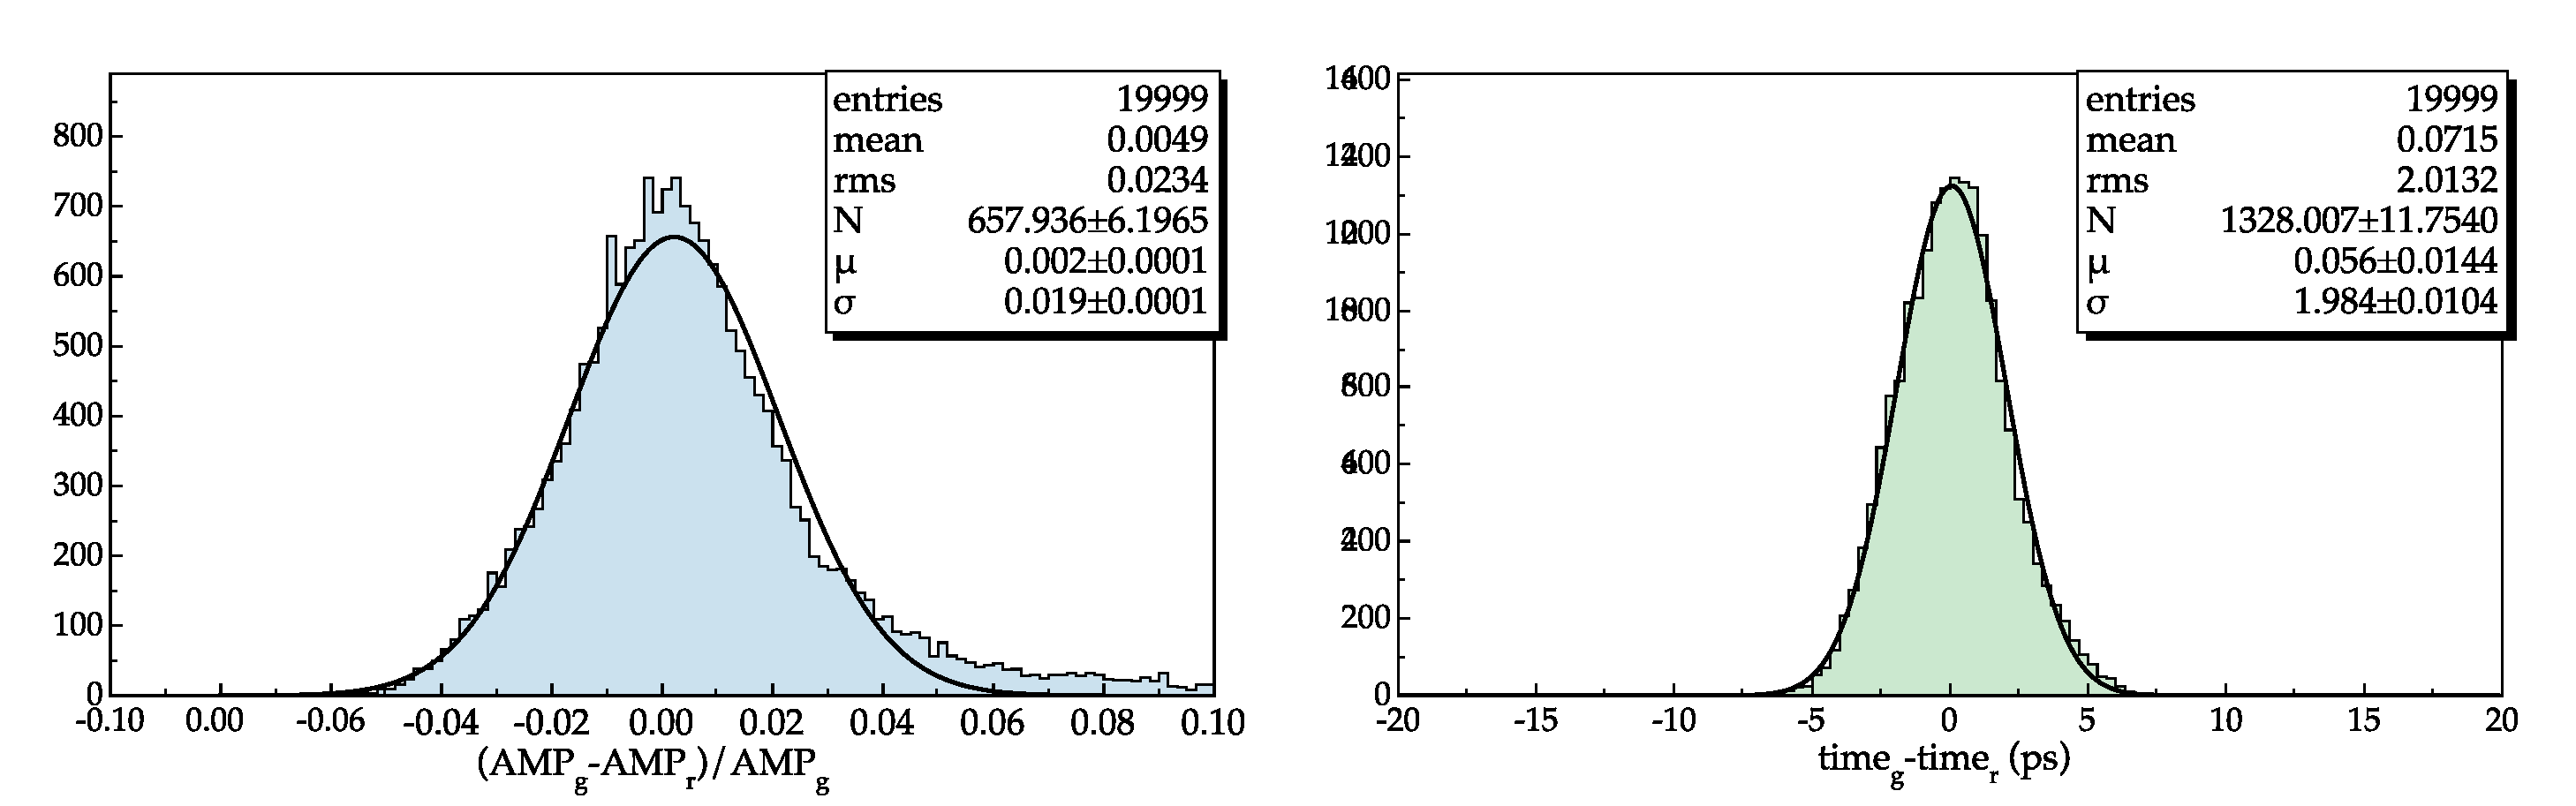
\includegraphics[width=0.9\columnwidth]{out_evaluate_csv_double_24.pdf}
\caption{The resolution of the pulse integrals (double pulses). The integral of the pulse is compared to the integral calculated from decompressed pulses (on the right), and the time calculated from the original pulse is compared to the time calculated from the decompressed pulse.} 
\label{fig:results_dp_48_res}
\end{figure}

To improve the two-pulse data compression a different network architecture was considered. Traditionally the autoencoders are constructed in a way that each subsequent layer starting from the input layer is smaller in size. This can potentially cause some issues when the input vector is not large enough, where the subsequent layer already has to find a more compact representation of the input. 
Following the logic from convolutional networks, one would expect that the layer following the input layer should be larger to be able to encode some different features from the input vector into much larger space, before trying to compress it. Inspired by this logic the network architecture was changed to have a larger hidden layer to follow the input layer in the network and changed the architecture to 
{\bf [48,96,48,24,12,24,48,96,48] }, while keeping it symmetric for both the encoder and decoder sides. The new network was trained on the same training sample with double pulses from our previous test, and the results can be seen in Figure~\ref{results_dp_96.pdf}. 

\begin{figure}[h!]
\centering
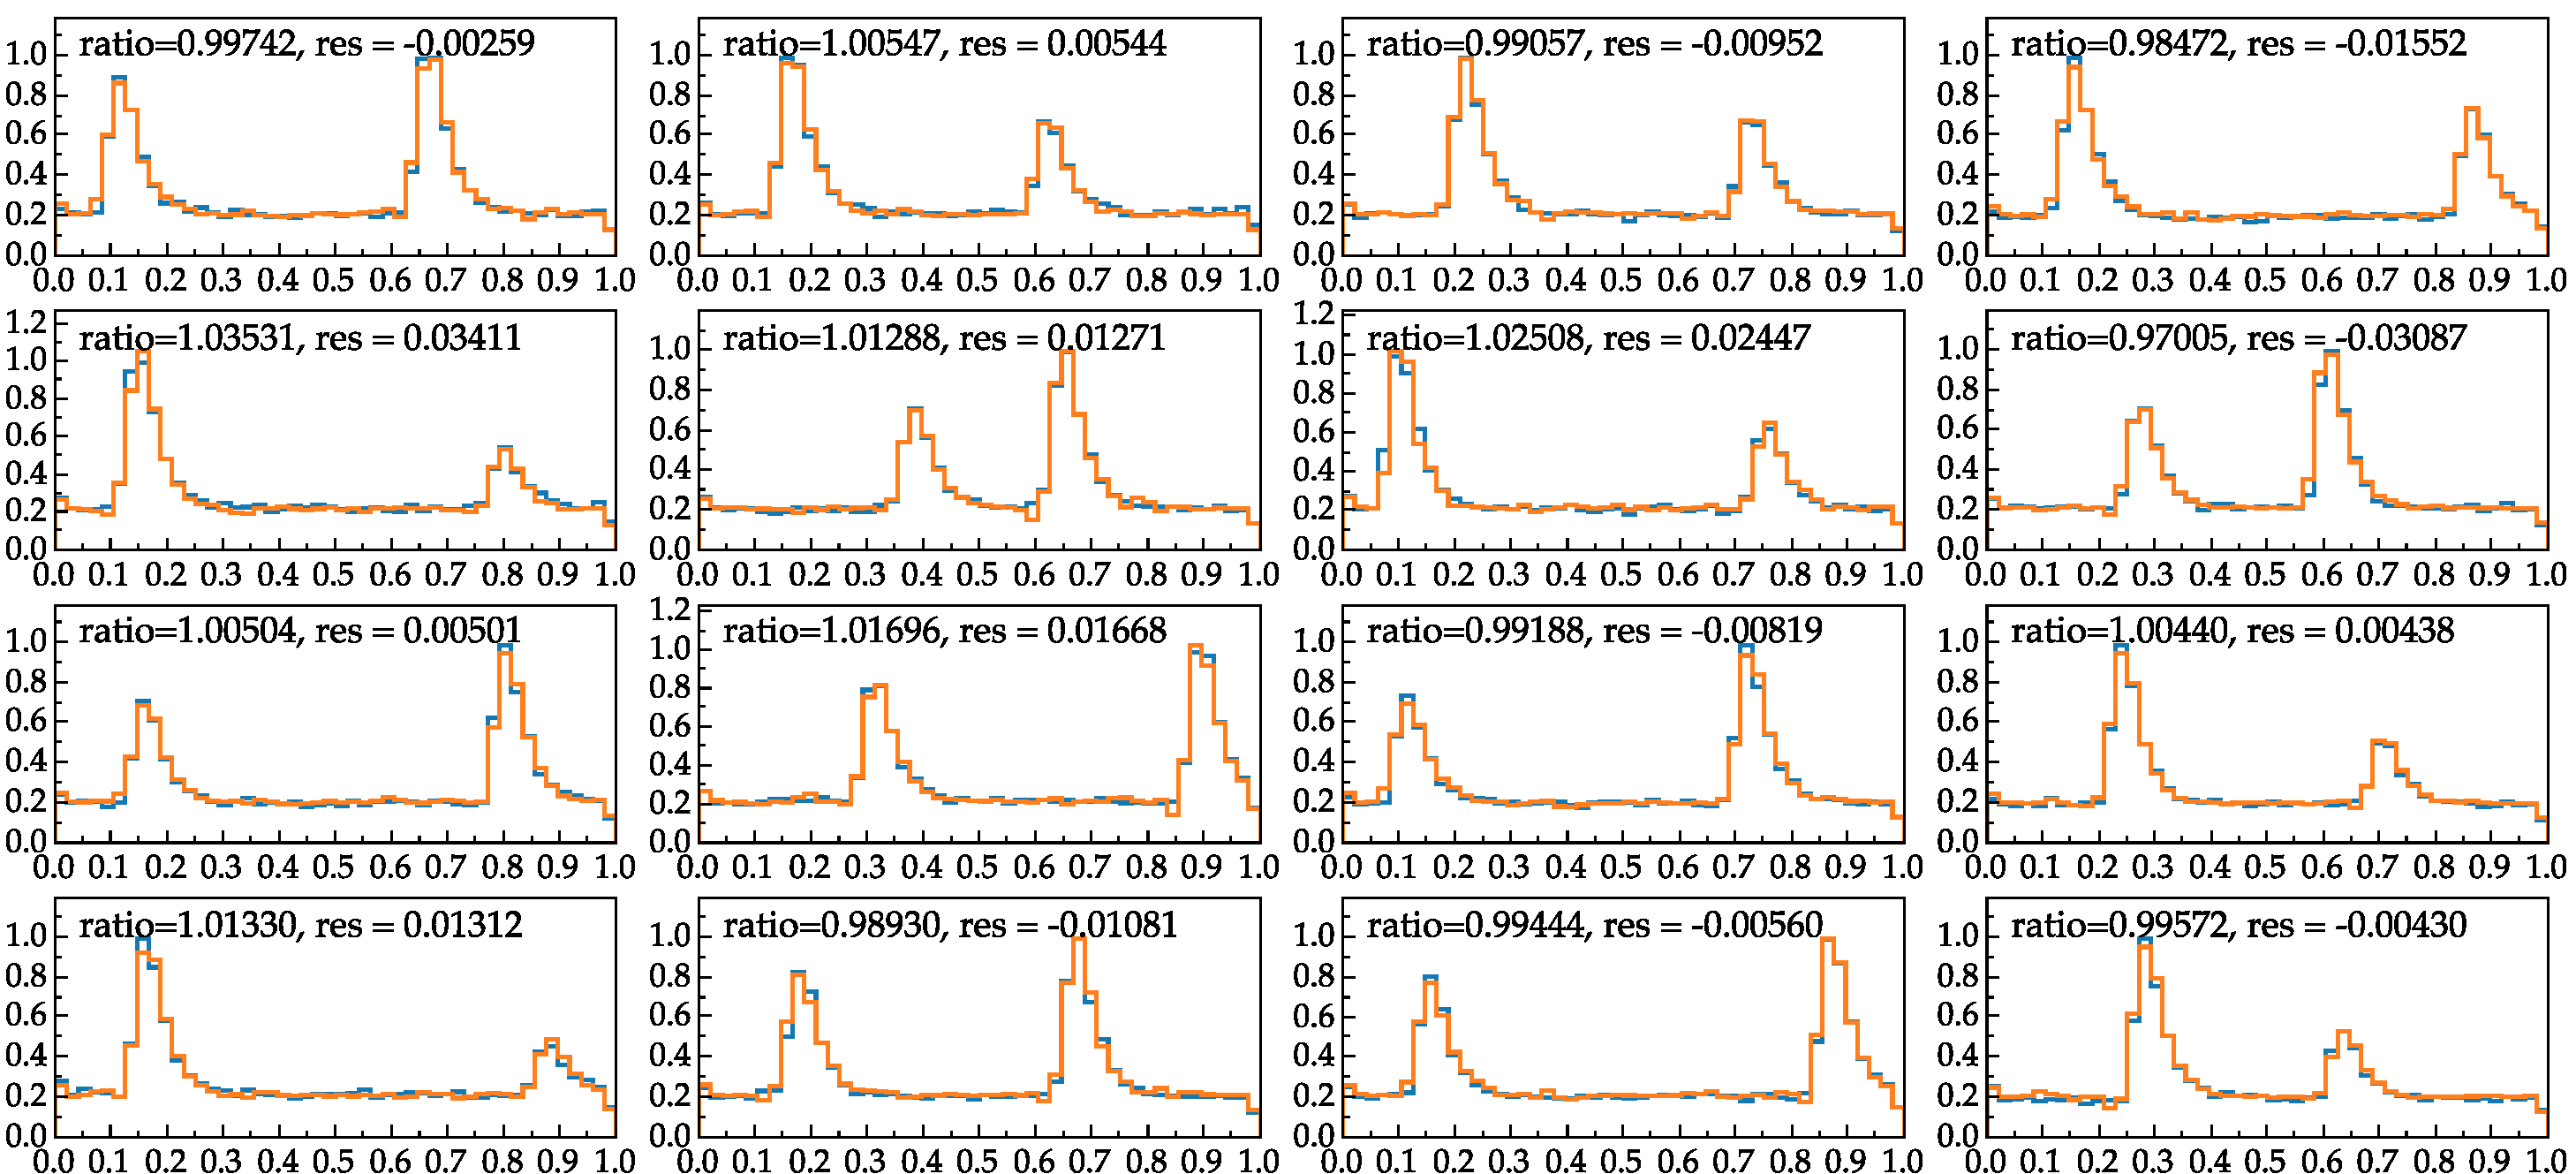
\includegraphics[width=0.9\columnwidth]{results_dp_96.pdf}
\caption{Generated double pulses plotted with the decompressed pulses overlayed. The compression is done with the improved auto-encoder [48,96,48,24,12,24,48.96,48] architecture. The data is produced by simulating a single pulse in the 48-bin region.} 
\label{fig:results_dp_96}
\end{figure}

The results show significant improvement in peak reconstruction from compressed latent space, where not only the peak positions are well reconstructed, but also the peak heights and withs have very close values to the original raw pulse. And the normalized difference of the peak integrals also shows significant improvements compared to the old network architecture and reaches a resolution of $1.4\%$.

\begin{figure}[h!]
\centering
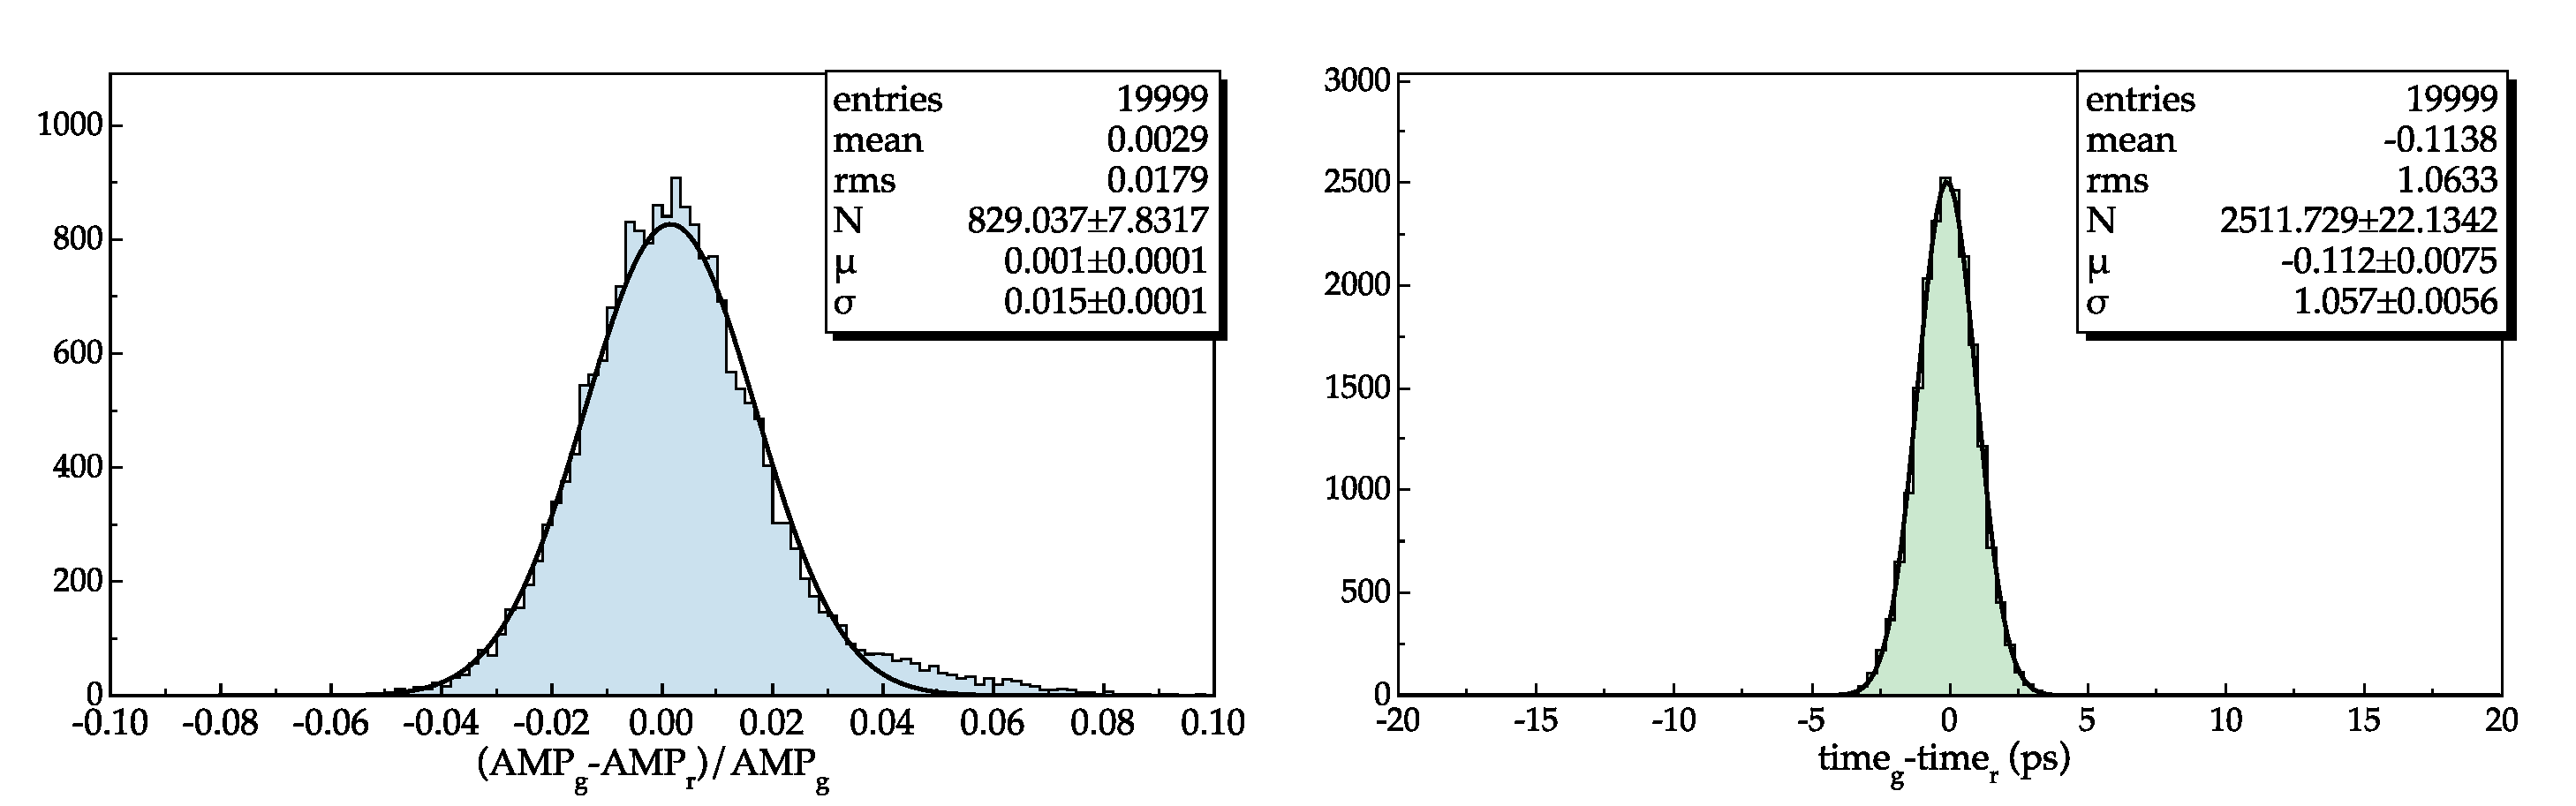
\includegraphics[width=0.9\columnwidth]{out_evaluate96_12_csv.pdf}
\caption{The resolution of the pulse integrals (double pulses). The integral of the pulse is compared to the integral calculated from decompressed (with network [48,96,48,24,12,24,48.96,48]) pulses (on the right), and the time calculated from the original pulse is compared to the time calculated from the decompressed pulse.} 
\label{fig:results_dp_96_res}
\end{figure}

